\chapter{Woody Classifier-based Latency Estimation}
\section{Latency estimation and correction}
\todo{check earlier draft alignment paper}
\todo{check deleted paragraphs in jitter paper}
\section{Classifier-based Latency Estimation}
\section{Classifier-based Latency Estimation with Woody iterations}
\section{Simulation study}


\section{Introduction}
Single-trial ERP latency jitter introduces a problem in ERP analysis:
the \textit{smearing effect} occurs when aggregating over multiple identical
signals with different latencies.
A familiar example of this happens when averaging over jittered epochs for ERP
analysis.
In the presence of jitter, the shape and amplitude of the average do not
reflect the properties of the original signal.
As the smearing effect reduces the amplitude of the average,
it negatively impacts the signal-to-noise ratio (SNR).
The smearing effect equally impacts the SNR of information captured by a
classifier's parameters when training with a procedure that does not account for
this jitter, and thus also affects its performance~\cite{Thompson2012}.
Hence, effective latency estimation and jitter compensation can contribute to higher
decoding performance.
%In this work, we propose a latency estimation and alignment strategy based on
%the method proposed by \cite{Thompson2012}.

The most straightforward latency estimation method is \textit{peak picking}.
Peak picking determines the latency of an ERP as the time point of its maximum
(or minimum for negative components) amplitude relative to stimulus
onset.
While easy to implement, this method does not perform well in low or negative
SNR conditions because of the risk of picking a noise-related peak, unless
combined with strong filtering in the space, time or frequency
domains~\cite{Avanzo2011,Arico2014,TREDER2016279,Ouyang2017}.
The aforementioned analysis and performance prediction method proposed
by \cite{Arico2014} estimates the single-trial P3 latencies of attended
epochs by P3 peak-picking after filtering in the time-frequency domain, and
corrects for jitter by temporally aligning all target epochs to the average
latency, i.e., by shifting the epochs in time such that the P3 peaks all fall
at the same time instance.
Due to the risk of picking noise peaks, template matching is generally
preferred.
Woody's algorithm~\cite{woody1967characterization} is a simple and performant
latency estimation method that is considered to be among
the most performant ones~\cite{Ouyang2017}.
Woody's scheme starts with a template that approximates the expected response,
e.g. the average target ERP, and iteratively enhances the SNR of this template by determining at
each iteration the time point of maximum cross-correlation of the template
with all single-trial ERPs, and aligning them based on these latencies to form
the template for the next iteration.
The final, enhanced template can then be cross-correlated again to retrieve an
accurate estimation of single-trial latencies.
Similar to peak-picking, cross-correlation template matching can be combined
with a spatial filter such as XDAWN~\cite{souloumiac2013improved} or a
spatiotemporal filter \cite{Iturrate2014}.
More recent work achieves good performance in latency estimation using residue
iteration~\cite{Ouyang2017}, genetic
algorithms~\cite{Pelo2018}, a hidden process model~\cite{Kim2020} or
graph-based network analysis~\cite{Dimitriadis2018}.

When multiple clusters of ERP components are not time-locked to
each other, aligning to the latency of one cluster might introduce more jitter
in other component clusters, further decreasing the SNR~\cite{Ouyang2020}.


Finally, algorithms that use time
warping-based methods instead of explicit ERP component latency estimation can
also overcome the smearing problem.
Examples that have been applied to ERPs are Dynamic Time
Warping~\cite{Casarotto2005,486255,wang2001warp,Zoumpoulaki2015},
Correlation-Optimized Warping~\cite{Skov2006}, or Fast Variational
Alignment~\cite{Flotho2021}. Since these methods are fundamentally
different from latency estimation methods,
we will not further consider them in this work.

Most of these methods suffer from a common drawback: they cannot be used in a
decoding scheme to improve performance for incoming epochs with unknown
class labels that contain either a target or non-target ERP response.
They can be used offline on a set of labeled epochs for testing hypotheses
concerning latency and jitter, for aligning templates, or for BCI performance
prediction, but not for ERP classification.
While some of the aforementioned methods could be adapted to perform
classification tasks, few studies investigate how to exploit this latency estimation
for jitter-resistant decoding.
\cite{hardiansyah2020single} incorporated single-trial latencies in
classification by peak-picking within a given
ERP time window, unaware of the class of the epoch under investigation.
The Classifier-Based Latency Estimation (CBLE) algorithm introduced
by \cite{Thompson2012} also explicitly applies latency estimation in a
decoding setting.
\cite{Thompson2012} initially formulated CBLE as an off-line performance prediction method.
Later, its output was successfully adapted to compensate for jitter to improve decoder performance%
~\cite{Mowla2017,Zisk2022}.

Time series classification algorithms~\cite{Abanda2019}
that are robust to jitter can be used in a decoding setting,
but, in general, have scarcely been applied to ERP decoding.
Data augmentation involving jittering the training
data~\cite{Krell2018,Zisk2022} and Riemannian Geometry methods using spatial
covariances as features~\cite{Aydarkhanov2020} have both been shown
to perform well in the presence of ERP jitter.
In this work, we opted to apply CBLE because it has successfully been applied to
classify jittered ERPs.
We adapt the CBLE to an iterative method akin to Woody's scheme that can better
compensate for jitter, to improve covert VSA decoding performance.

\section{Materials and Methods}
\subsection{Decoders}
\subsubsection{Classifier-based Latency Estimation}
\label{sec:cble}

Consider a training set of $N$ EEG epochs with $C$ channels of $S$
samples $\{\mat{X}_n^\mathrm{train} \in \mathbb{R}^{C\times S}\}_{n=1}^N$
with corresponding training labels $\mathbf{l^\mathrm{train}} \in \{\mathrm{target},
	\textrm{non-target}\}_{n=1}^N$, and a
similar testing set of $M$ epochs $\{\mat{X}_m^\mathrm{test} \in
	\mathbb{R}^{C\times S}\}_{m=1}^M$.
We assume that the sampling period is $T$, i.e. that the sample with index $s$ is sampled at time $sT$.
In the following, we use the matrix slicing notation to denote row or column intervals extracted from a matrix.
For instance, $\mat{X}[:,s_1:s_2]$ denotes all columns of $\mat{X}$ with indices between $s_1$ (included) and $s_2$ (excluded).

CBLE, summarized in Algorithm~\ref{alg:cble}, works by training a
\textit{first-stage} classifier $\mathcal{C}(\theta,f)$
defined within a time period $[s_1:s_2]$ with a set of parameters $\theta$ and a
decision function $f(\mat{X}[:,s_1:s_2],\theta) \rightarrow
y$ outputting a classification score $y\in\mathbb{R}$ for a given epoch $\mat{X}$,
such that
\begin{equation}
  \theta = \mathrm{train}_\mathcal{C}(\{\mat{X}_n^\mathrm{train}[:,s_1:s_2]\}_{n=1}^N,\mathbf{l}^\mathrm{train})
  \label{eq:cble-train}
\end{equation}
Then,
%instead of applying the classifier directly to an unseen, cropped
%testing epoch $\mat{X}[:,s_1:s_2]$ and obtaining a single score value $y$,
$f$ can be applied to all (possibly overlapping) slices of length $s_2-s_1$ of
an epoch $\mat{X}$, resulting in a vector of score values
$\mathbf{y}=[y_1\,\ldots\,y_R]^T \in\mathbb{R}^R$ such that
\begin{equation}
  y_s = f(\mat{X}[:,s:s+(s_2-s_1)],\theta)\quad \forall s\in 1,\ldots,R
	\label{eq:score}
\end{equation}
with $R = S-(s_2-s_1)$.
To leverage CBLE for ERP classification, the score vectors $\mathbf{y}$ can be
arranged in matrices $\mat{Y}^\mathrm{train}\in\mathbb{R}^{N\times R}$ and $\mat{Y}^\mathrm{test}\in\mathbb{R}^{M\times R}$.
These can be further classified by training a \textit{second-stage} classifier on
$\mat{Y}^\mathrm{train}$ and class labels $\mathbf{l}^\mathrm{train}$.
However, the resulting score-over-time vectors per epoch still suffer from jitter.
For classification, we follow the approach of \cite{Mowla2017}, using a
maximum-level hierarchical Daubechies-4 wavelet transform to reduce
dimensionality before classification with the second-stage classifier.
In the CBLE-decoder, it is this wavelet transform that decreases the sensitivity
to latency differences, actively compensating for ERP latency jitter.

When using a simple spatiotemporal linear classifier as first-stage classifier,
CBLE is equivalent to the first iteration of Woody's algorithm with the
spatiotemporal classifier weights as template.
\cite{Thompson2012}, \cite{Mowla2017} and \cite{Mowla2020} show
that CBLE is relatively independent of the first-stage classifier for BCI
accuracy prediction and for ERP classification.
Therefore, we opt to use the variant of Linear Discriminant Analysis with block-Toeplitz
regularized covariance matrix (tLDA) proposed by \cite{Sosulski2022}, as the first-stage
classifier and logistic regression as second stage.

\subsubsection{Robust CBLE latency features}
\label{sec:robust-latency}
The ERP decoding method based on CBLE introduced by \cite{Mowla2017} does
not make use of the extracted latencies, only passing score matrix $\mat{Y}$ on
to the second-stage classifier.
%Furthermore, previous CBLE works~\cite{Thompson2012,Mowla2020} only used these
%latencies to correlate them with neurophysiological processes or to predict
%decoder performance.
We noticed that, while CBLE performance was unaffected, the classification
performance of our proposed method can be improved if the estimated
latencies are also made available as features to the second-stage classifier,
after a square transform for linear separability~\cite{Thompson2012}.

These latency features give rise to the following issue when
classifying unseen data.
The CBLE latency estimate is defined only for target epochs as
$s_\mathrm{target}=\argmax_s{y_s}$.
This is the point in time where the target class reaches largest separation
from the background noise and non-target class, indicating the target ERP is
most likely to occur here.
However, in a classifier test phase, it is not known a priori whether an
unseen epoch is a target or a non-target epoch.
This problem is solved by defining an estimated latency per class
$s_\mathrm{target}$ and $s_\mathrm{non-target}$ for every epoch,
regardless of its actual class.
The estimated class latencies can then be used as features  for training and
testing the second-stage classifier.
This way, the latencies of the testing data can be presented to the second-stage
classifier without knowledge of the testing data class labels, making them
useful in decoding.

In a similar manner to the target latency, the non-target latency could be defined
as~$s_\mathrm{non-target}=\argmin_s{y_s}$.
However, this is problematic since it is not evident how to estimate
latency of e.g. a P3 ERP component for a non-target epoch, since the
non-target class is characterized by the absence of this component.
%\footnote{Depending on the stimulation and experimental design, ERP components can be present in one experimental
%	condition or class and missing in another, or appear in multiple classes
%	at different amplitudes. In the latter case, it could be possible
%	to estimate the latency of an ERP in the conditions where it appears, but if
%	its amplitude is lower or negligible in some conditions, latency estimates
%	will be less accurate, hence this case is still problematic.}.
In fact, $y$ can have multiple local minima or entirely lack distinct peaks for
non-targets, rendering the minimum estimate meaningless.

Instead, we opt for a more robust, probabilistic definition of class latencies.
This robust estimation method yields latencies that
\begin{enumerate*}[label=(\arabic*)]
  \item are more meaningful as input for the second-stage
    classifier, and
  \item lead to smoother convergence in our proposed iterative alignment scheme
    for WCBLE, which heavily relies on exact latency estimation.
\end{enumerate*}
Assume classifier $\mathcal{C}(\theta,f,\Pr)$ now can also output a probability
per class $\Pr(l|
\mat{X}[:,s_1:s_2:)], \theta)$ for a given epoch $\mat{X}$, a feature of many
common classifiers.
Analogous to equation~\ref{eq:score}, we can now write
\begin{equation}
\Pr(\mat{X},\theta,l,s) = \frac{1}{R}\Pr(\mat{X}[:,s:s+(s_2-s_1)],\theta,l)
  \quad \forall \quad s\in 1,\ldots,R
	\label{eq:prob}
\end{equation}
The latency features assuming the epoch belongs to a given class
$l\in\{\textrm{target},\textrm{non-target}\}$ are then defined as the median of
the corresponding  distributions
\begin{equation}
  s_l =\mathrm{median}\left[\Pr(s|\mat{X},\theta,l) \right] \\
  \label{eq:prob-latency}
\end{equation}
Note that $  \Pr(s|\mat{X},\theta,\textrm{non-target}) =1-
  \Pr(s|\mat{X},\theta,\mathrm{target})$.
The median of the probability distribution over time is more robust to
outliers and noise than the maximum or minimum score.
For the non-target case, the median approach tends towards the center of a
near-uniform distribution, resulting in a more consistent latency estimate over
trials as compared to the minimum approach.

\subsubsection{Classifier-based Latency Estimation with Woody
	Iterations}
To improve performance over CBLE, we propose a new algorithm inspired both by
CBLE and the aforementioned Woody iteration scheme (WCBLE).
Instead of using CBLE to estimate the features of a second-stage classifier
directly, CBLE latency estimation is used as a step in a Woody iteration scheme.
While the Woody algorithm iteratively enhances the SNR of an ERP template to
cross-correlate with the data, WCBLE iteratively re-estimates the parameters of
the first-stage classifier.
To improve convergence and perform well in a classification setting, WCBLE
aligns both targets and non-targets to their corresponding estimated latencies.

The WCBLE algorithm is presented in Algorithm~\ref{alg:wcble}.
Its training phase is visualized in~Figure~\ref{fig:diagram-train}.
The initial training epochs $\{\mat{X}_n^{(1)}\}_{n=1}^N$ are set to $\{\mat{X}_n^\mathrm{train}\}_{n=1}^N$.
At every iteration, classifier $\mathcal{C}$ is trained like in CBLE:
\begin{equation}
  \theta^{(i)} =
  \mathrm{train}_\mathcal{C}(\{\mat{X}^{(i-1)}_n[:,s_1:s_2]\}_{n=1}^N,\mathbf{l}^\mathrm{train})
\end{equation}
Next, latency $s_{l_n}^{(i)}$ is determined for every epoch $\mat{X}^{(i)}$ corresponding
to its class label $l_n$ using equation~\ref{eq:prob-latency}.
Finally, the training epochs $\mat{X}^{(i+1)}$ for the next iteration are determined by aligning
each original training epoch to the latency $s_{l_n}^{(i)}$ corresponding to its respective class
label.
\begin{equation}
  \mat{X}^{(i+1)}_n = \mathrm{align}(\mat{X}_n^\mathrm{train}, s_{l_n}^{(i)}) \quad \forall \quad n=1,\ldots,N
\end{equation}
Aligning is performed by shifting and zero-padding the signal to the right if
the latency is negative relative to the time window onset, and to the left if
positive, by the difference between the latency and the window onset.
\begin{figure*}
	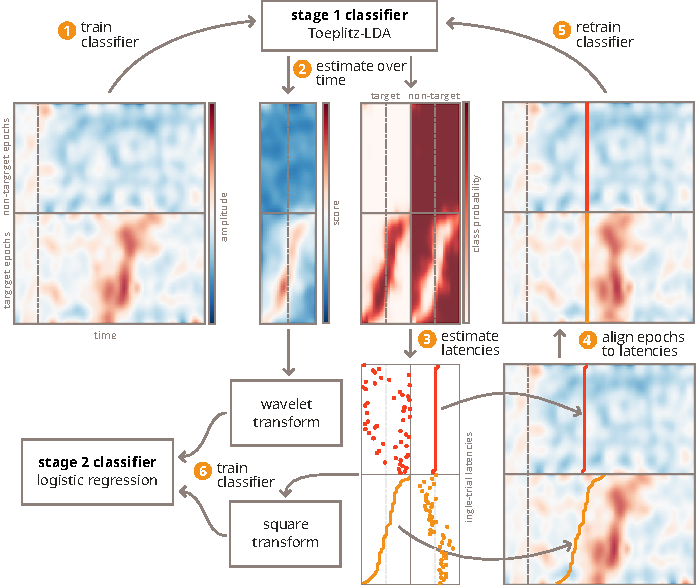
\includegraphics[width=\linewidth]{figures/wcble/figure1.pdf}
	\caption{Schematic representation of the Woody Classifier Based Latency
    Estimation training phase.
    (1) The first-stage spatiotemporal binary classifier is trained on a set of
    epochs.
    (2) It is	then applied to time-shifted copies of the epochs to obtain scores
    and class probabilities	over time.
    (3) The medians of these probability distributions are assumed the class
    latencies.
    (4) The epochs are aligned to their corresponding	class latencies by
    shifting in time such that all latencies fall at the same moment.
    (5) The spatiotemporal classifier is then retrained on the aligned epochs
    for a	next iteration.
    (6) After the iterative process halts, the scores and	latencies obtained
    from the last iteration are used to train the second-stage
		classifier.}
	\label{fig:diagram-train}
\end{figure*}
The process halts after a fixed amount of iterations or when the estimated set
of latencies has been encountered before, indicating it ended up in a loop.
In the end, the procedure should result in enhanced classifier parameters $\theta^*$,
closer to those when there would be no jitter between epochs.
Note that using the median approach for robust latency estimation results in a
smoother yet longer convergence process compared to the maximum/minimum approach.
We can then apply the classifier with enhanced parameters $\theta^*$ in a CBLE
manner to unseen epochs as illustrated in Figure~\ref{fig:diagram-eval} to obtain a
vector of scores over time as in~Section~\ref{sec:cble} and the estimated latencies as
in~Section~\ref{sec:robust-latency}.
\begin{figure*}
	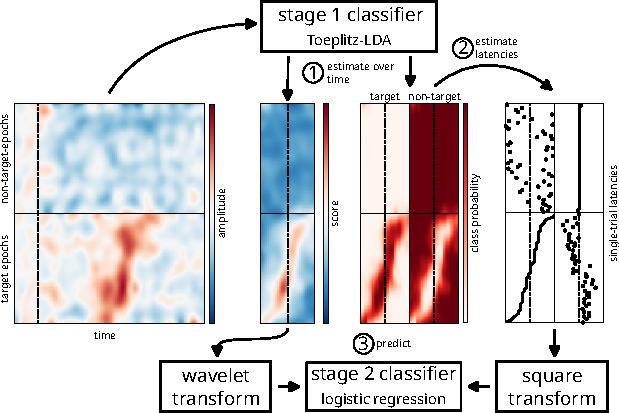
\includegraphics[width=\linewidth]{figures/wcble/figure2.pdf}
	\caption{Schematic representation of the Woody Classifier Based Latency
    Estimation test phase. (1) The
		first-stage	spatiotemporal binary classifier obtained from the training phase is
		applied to time-shifted copies of the epochs to obtain scores and class probabilities
		over time. (2) The medians of these probability distributions are assumed
		as the new class latencies. (3) The scores and class latencies are input to the
		trained second-stage classifier, which predicts the label of the epochs.}
	\label{fig:diagram-eval}
\end{figure*}
\section{Algorithms}

\begin{algorithm}[H]
	\textsc{Train}
	\smallskip \hrule \smallskip
	\textbf{Input:} $\{\mbfX_n^\mathrm{train}\}_{n=1}^N,
  \mathbf{l}^\mathrm{train}, \mathcal{C}(\cdot,f, \Pr), s_1, s_2$
  \begin{algorithmic}[1]
		\State $\theta \gets
			\mathrm{train}_\mathcal{C}(\{\mbfX_n^\mathrm{train}[:,s_1:s_2]\}_{n=1}^N,\mathbf{l})$
      \algorithmiccomment{Train stage 1}
		\For{$n=1\ldots N$}
      \algorithmiccomment{Feature extraction for stage 2}
		  \For{$s=1\ldots R$}
      \State $y_{n,s}^\mathrm{train} \gets f(\mbfX_n^\mathrm{train}[:,s:s+(s_2-s_1)],\theta)$
        \EndFor
        \State $s_{n,\mathrm{target}}^\mathrm{train} \gets
			    \mathrm{median}\left[Pr(s|\mbfX_n^\mathrm{train},\theta,\mathrm{target})\right]$
		    \State $s_{n,\mathrm{non-target}}^\mathrm{train}\gets
			    \mathrm{median}\left[Pr(s|\mbfX_n^\mathrm{train},\theta,\textrm{non-target})\right]$
    \EndFor
	\end{algorithmic}
  \textbf{Output:} $\theta,
  \mbfY^\mathrm{train},
  \mathbf{s}_\mathrm{target}^\mathrm{train},
  \mathbf{s}_\mathrm{non-target}^\mathrm{train}$
	\smallskip \hrule \smallskip
	\textsc{Evaluate}
	\smallskip \hrule \smallskip
	\textbf{Input:} $\{\mbfX_m^\mathrm{test}\}_{m=1}^N, \mathcal{C}(\theta,f, \Pr), s_1, s_2$
  \begin{algorithmic}[1]
		\For{$m=1\ldots M$}
      \algorithmiccomment{Feature extraction for stage 2}
		  \For{$s=1\ldots R$}
      \State $y_{m,s}^\mathrm{test} \gets f(\mbfX_n^\mathrm{test}[:,s:s+(s_2-s_1)],\theta)$
        \EndFor
        \State $s_{m,\mathrm{target}}^\mathrm{test} \gets
			    \mathrm{median}\left[Pr(s|\mbfX_m^\mathrm{test},\theta,\mathrm{target})\right]$
		    \State $s_{m,\mathrm{non-target}}^\mathrm{test}\gets
			    \mathrm{median}\left[Pr(s|\mbfX_m^\mathrm{test},\theta,\textrm{non-target})\right]$
    \EndFor
	\end{algorithmic}
  \textbf{Output:} $\mbfY^\mathrm{test},
  \mathbf{s}_\mathrm{target}^\mathrm{test},
  \mathbf{s}_\mathrm{non-target}^\mathrm{test}$

	\caption{Classifier-Based Latency Estimation}
	\label{alg:cble}
\end{algorithm}

\newpage
\begin{algorithm}[H]
	\textsc{Train}
	\smallskip \hrule \smallskip
	\textbf{Input:} $\{\mbfX_n^\mathrm{train}\}_{n=1}^N, \mathbf{l},
		\mathcal{C}(\cdot,f,\Pr), s_1, s_2$
	\begin{algorithmic}[1]
		\State $\mbfX'_n \gets \mbfX^\mathrm{train}_n \quad \forall \quad n=1\ldots
    N$
      \algorithmiccomment{Train stage 1}
		\Repeat
		\State $\theta^* \gets \mathrm{train}_\mathcal{C}(\{\mbfX'_n[:,s_1:s_2]\}_0^{N-1},\mathbf{l}$
		\For{$n=1\ldots N$}
    \State  $s_n \gets
			    \mathrm{median}\left[Pr(s|\mbfX_n',\theta^*,l_n)\right]$
		\State $\mbfX'_n \gets \mathrm{align}(\mbfX^\mathrm{train}_n, s^*_n)$
		\EndFor
    \Until{convergence or maximum iterations reached}
    \For{$n=1\ldots N$}\algorithmiccomment{Feature extraction for stage 2}
		  \For{$s=1\ldots R$}
      \State $y_{n,s}^\mathrm{train} \gets
      f(\mbfX_n^\mathrm{train}[:,s:s+(s_2-s_1)],\theta^*)$
        \EndFor
        \State $s_{n,\mathrm{target}}^\mathrm{train} \gets
			    \mathrm{median}\left[Pr(s|\mbfX_n^\mathrm{train},\theta^*,\mathrm{target})\right]$
		    \State $s_{n,\mathrm{non-target}}^\mathrm{train}\gets
			    \mathrm{median}\left[Pr(s|\mbfX_n^\mathrm{train},\theta^*,\textrm{non-target})\right]$
    \EndFor

	\end{algorithmic}
	\textbf{Output:} $\theta^*,
  \mbfY^\mathrm{train},
  \mathbf{s}_\mathrm{target}^\mathrm{train},
  \mathbf{s}_\mathrm{non-target}^\mathrm{train}$

	\smallskip \hrule \smallskip
	\textsc{Evaluate}
	\smallskip \hrule \smallskip
	\textbf{Input:} $\{\mbfX_m^\mathrm{test}\}_{m=1}^N, \mathcal{C}(\theta^*,f, \Pr), s_1, s_2$
  \begin{algorithmic}[1]
		\For{$m=1\ldots M$}\algorithmiccomment{Feature extraction for stage 2}
		  \For{$s=1\ldots R$}
      \State $y_{m,s}^\mathrm{test} \gets
      f(\mbfX_n^\mathrm{test}[:,s:s+(s_2-s_1)],\theta^*)$
        \EndFor
        \State $s_{m,\mathrm{target}}^\mathrm{test} \gets
			    \mathrm{median}\left[Pr(s|\mbfX_m^\mathrm{test},\theta^*,\mathrm{target})\right]$
		    \State $s_{m,\mathrm{non-target}}^\mathrm{test}\gets
			    \mathrm{median}\left[Pr(s|\mbfX_m^\mathrm{test},\theta^*,\textrm{non-target})\right]$
    \EndFor
	\end{algorithmic}
  \textbf{Output:} $\mbfY^\mathrm{test},
  \mathbf{s}_\mathrm{target}^\mathrm{test},
  \mathbf{s}_\mathrm{non-target}^\mathrm{test}$
	\caption{Classifier-Based Latency Estimation with Woody Iterations}
	\label{alg:wcble}
\end{algorithm}
